\subsection{Distance controller}
A distance controller will now be designed, to complement the angular controller.
As concluded in \todo{secref}, a deviation from the planned line, will cause the vehicle to drive at a parallel line, next to the planned. The deviation will be calculated from the position provided by the GoT system. As the deviation is a function of the error angle integrated over time it is assumed, that a P controller will be sufficient to handle this function, just as in the Angular controller. The controller will therefore be based on a P controller, and iterated until results are satisfactory. 

As real-world test data is not available, caused by the magnetometer not working in the room with the GoT system installed, the controller will be designed and simulated in Simulink. As a starting point, the proportional gain will be set at 1, and the controller will be designed based on bode plots.

The proposed controlling scheme can be seen in \figref{SteeringSimulink}

\begin{figure}[H]
\centering
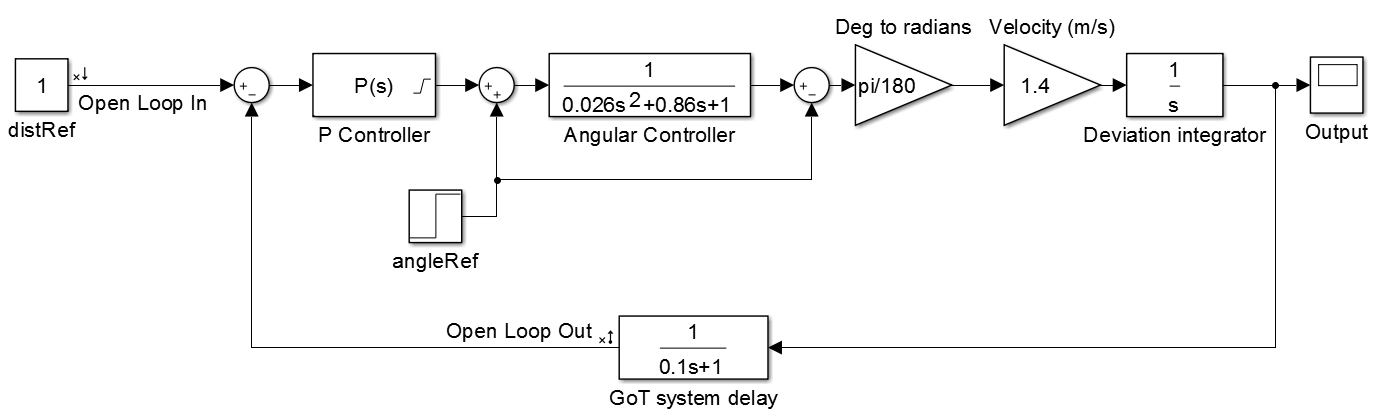
\includegraphics[width=\textwidth]{figures/SteeringSimulink1.png} 
\caption{Initial Distance Controller}
\label{SteeringSimulink}
\end{figure}

\begin{figure}[H]
  \centering
 	%Trim margins @:   left        bottom       right       top
 	\adjustbox{ trim = {.15\width} {.30\height} {.15\width} {.30\height}, clip }
  {
    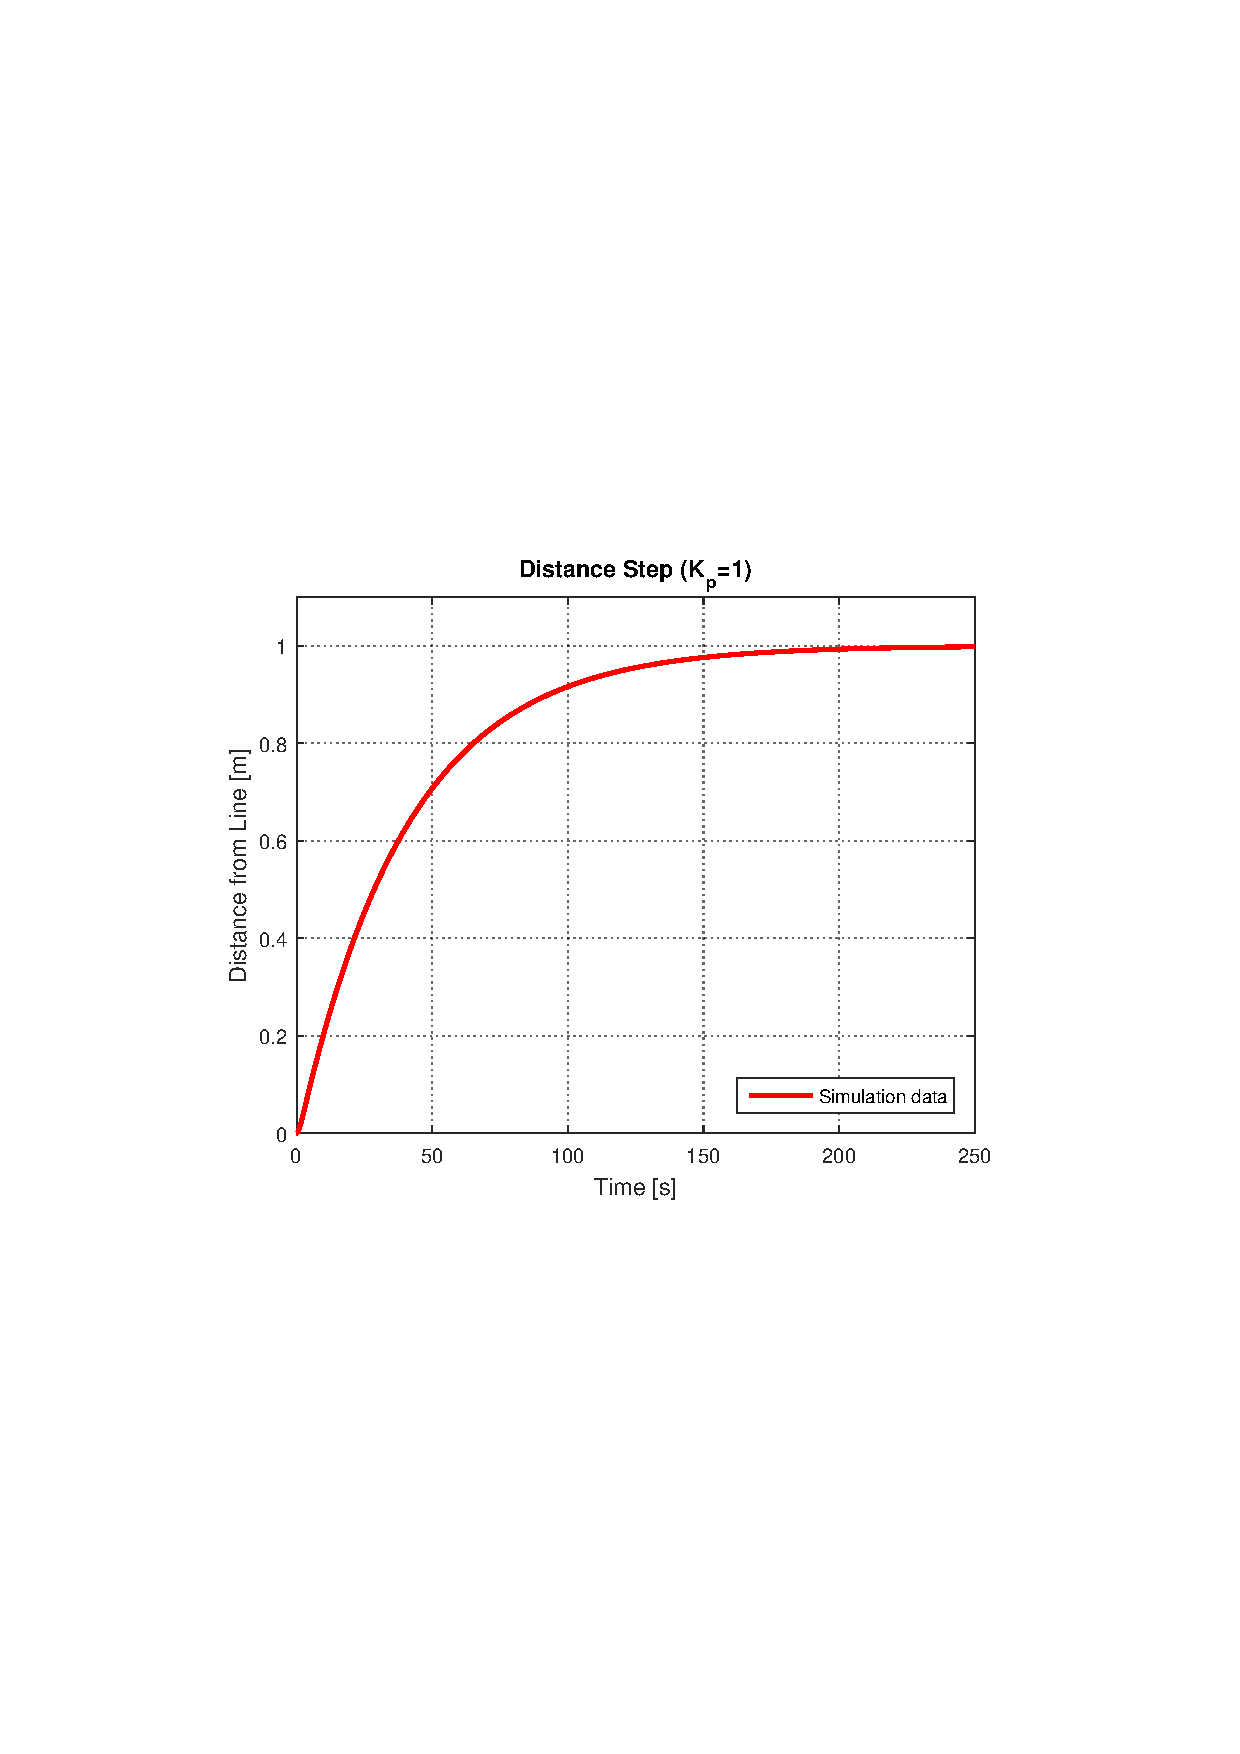
\includegraphics[width=1.4\textwidth]{figures/distanceStep1.pdf}
  }
  \caption{A plot illustrating a simulated step-response of the approximated velocity model (the blue line) and a measured step-response of the vehicle (the red line).}
  \label{SimulationSteeringP1}
\end{figure}
\begin{figure}[H]
  \centering
 	%Trim margins @:   left        bottom       right       top
 	\adjustbox{ trim = {.15\width} {.30\height} {.15\width} {.30\height}, clip }
  {
    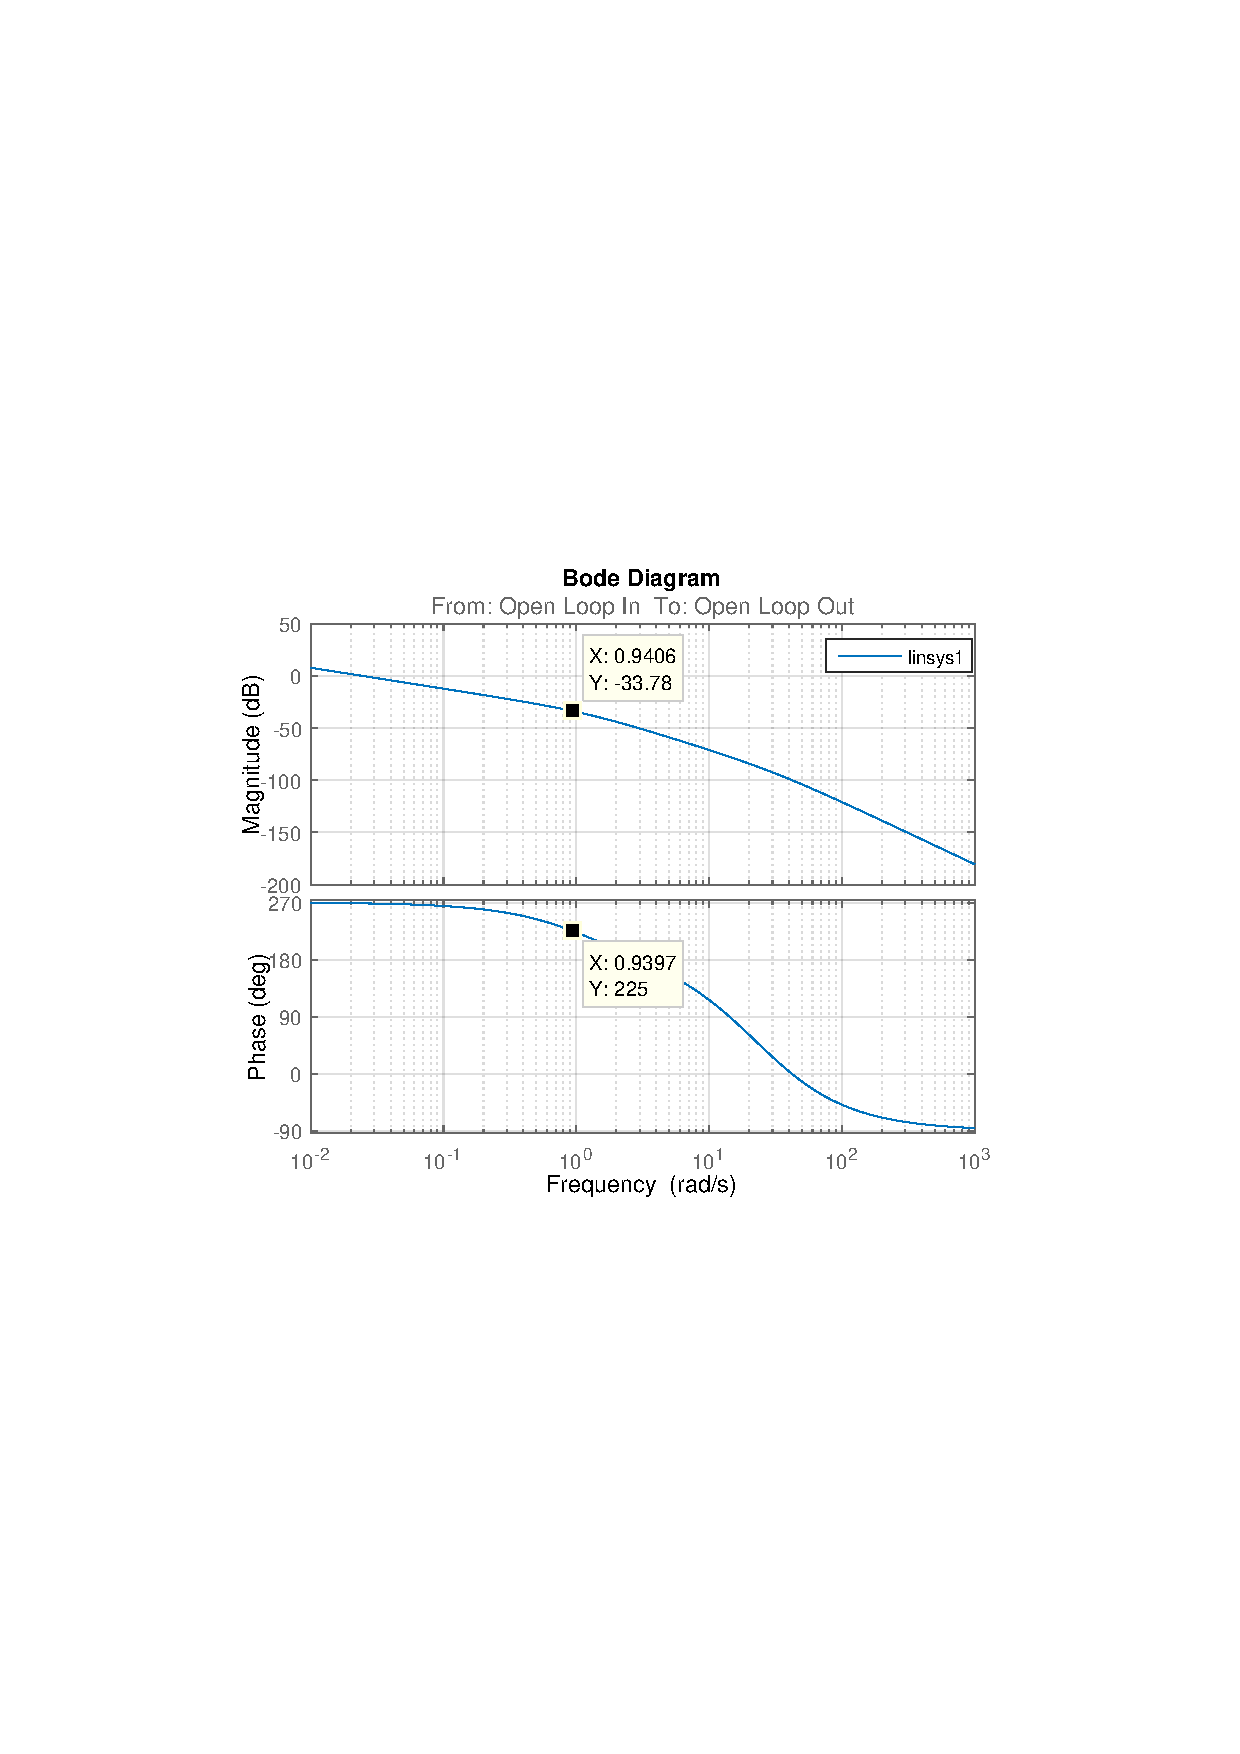
\includegraphics[width=1.4\textwidth]{figures/distanceBode1.pdf}
  }
  \caption{A plot illustrating a simulated step-response of the approximated velocity model (the blue line) and a measured step-response of the vehicle (the red line).}
  \label{SimulationSteeringB1}
\end{figure}
\begin{figure}[H]
  \centering
 	%Trim margins @:   left        bottom       right       top
 	\adjustbox{ trim = {.15\width} {.30\height} {.15\width} {.30\height}, clip }
  {
    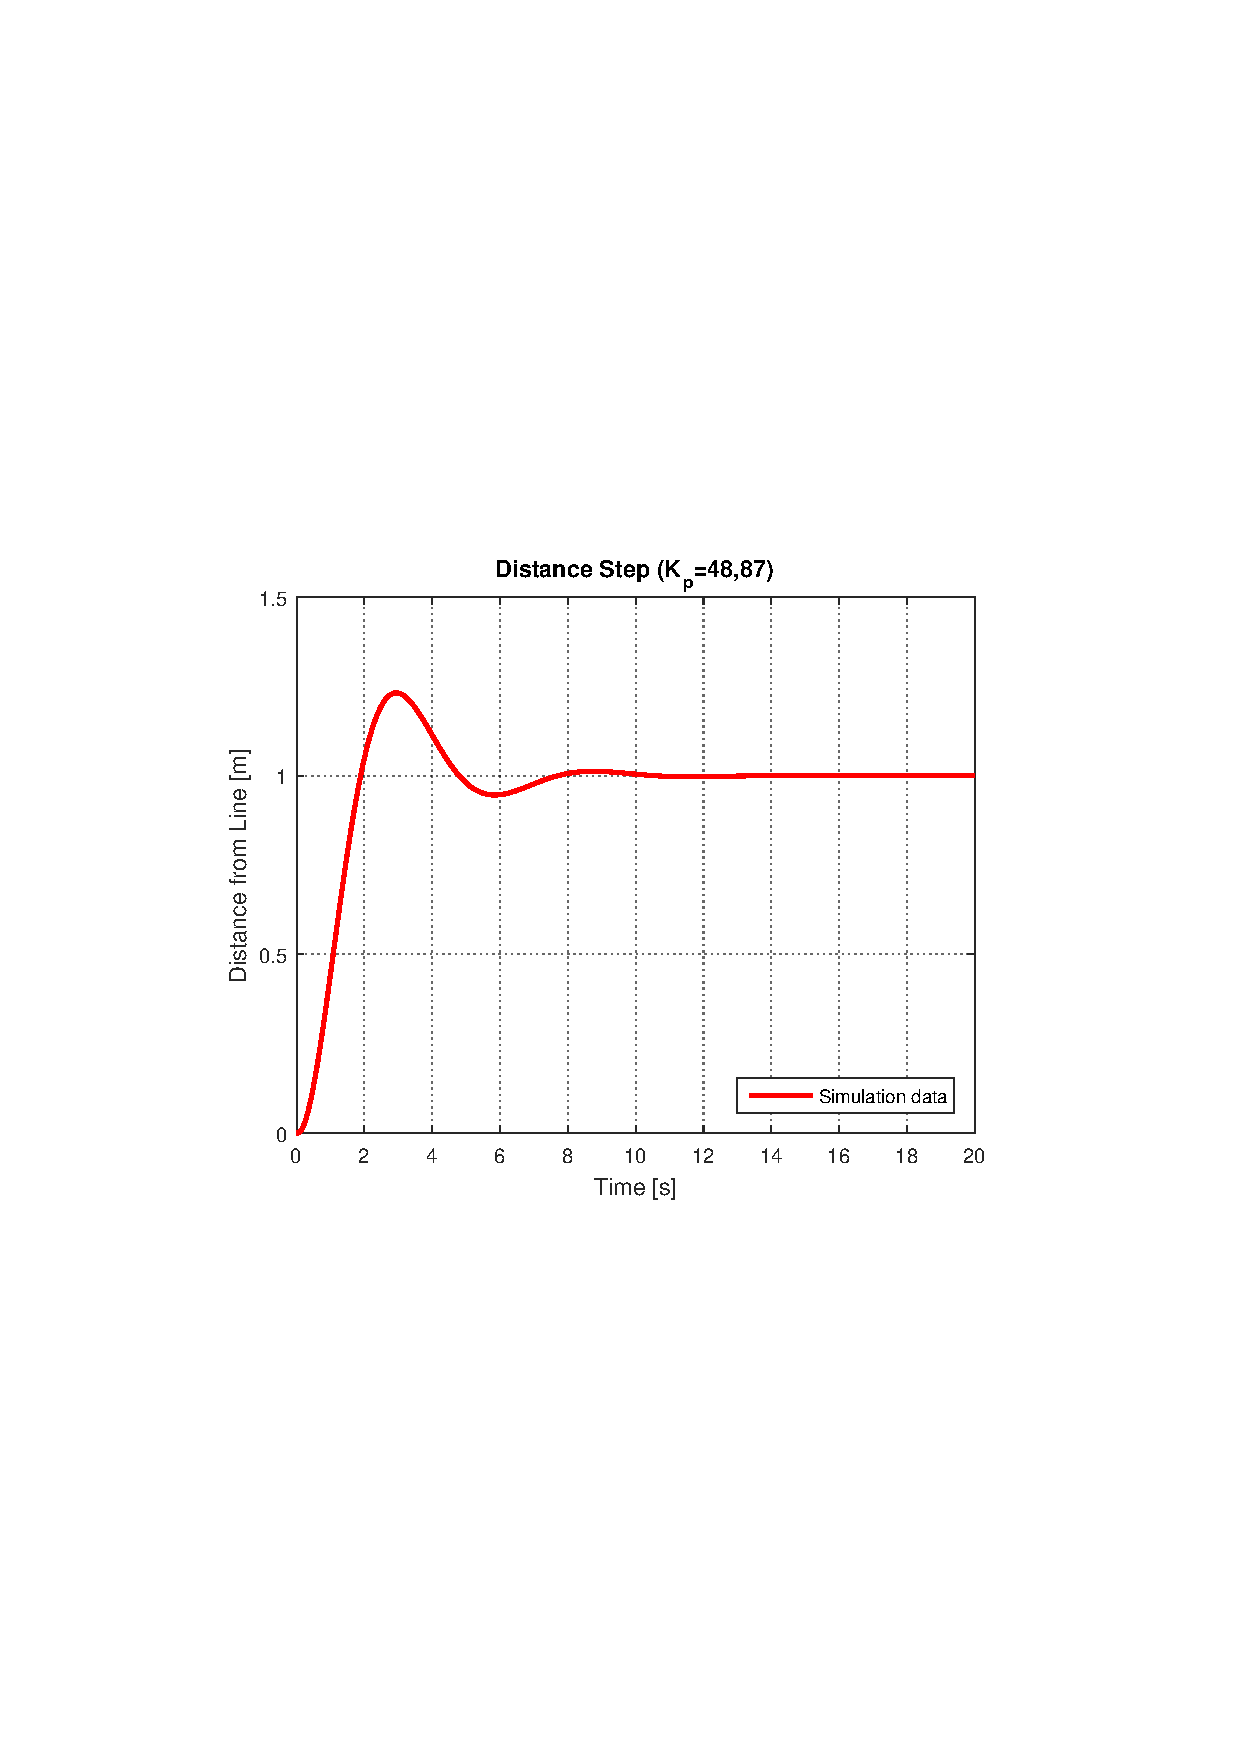
\includegraphics[width=1.4\textwidth]{figures/distanceStep2.pdf}
  }
  \caption{A plot illustrating a simulated step-response of the approximated velocity model (the blue line) and a measured step-response of the vehicle (the red line).}
  \label{SimulationSteeringP2}
\end{figure}
\begin{figure}[H]
  \centering
 	%Trim margins @:   left        bottom       right       top
 	\adjustbox{ trim = {.15\width} {.30\height} {.15\width} {.30\height}, clip }
  {
    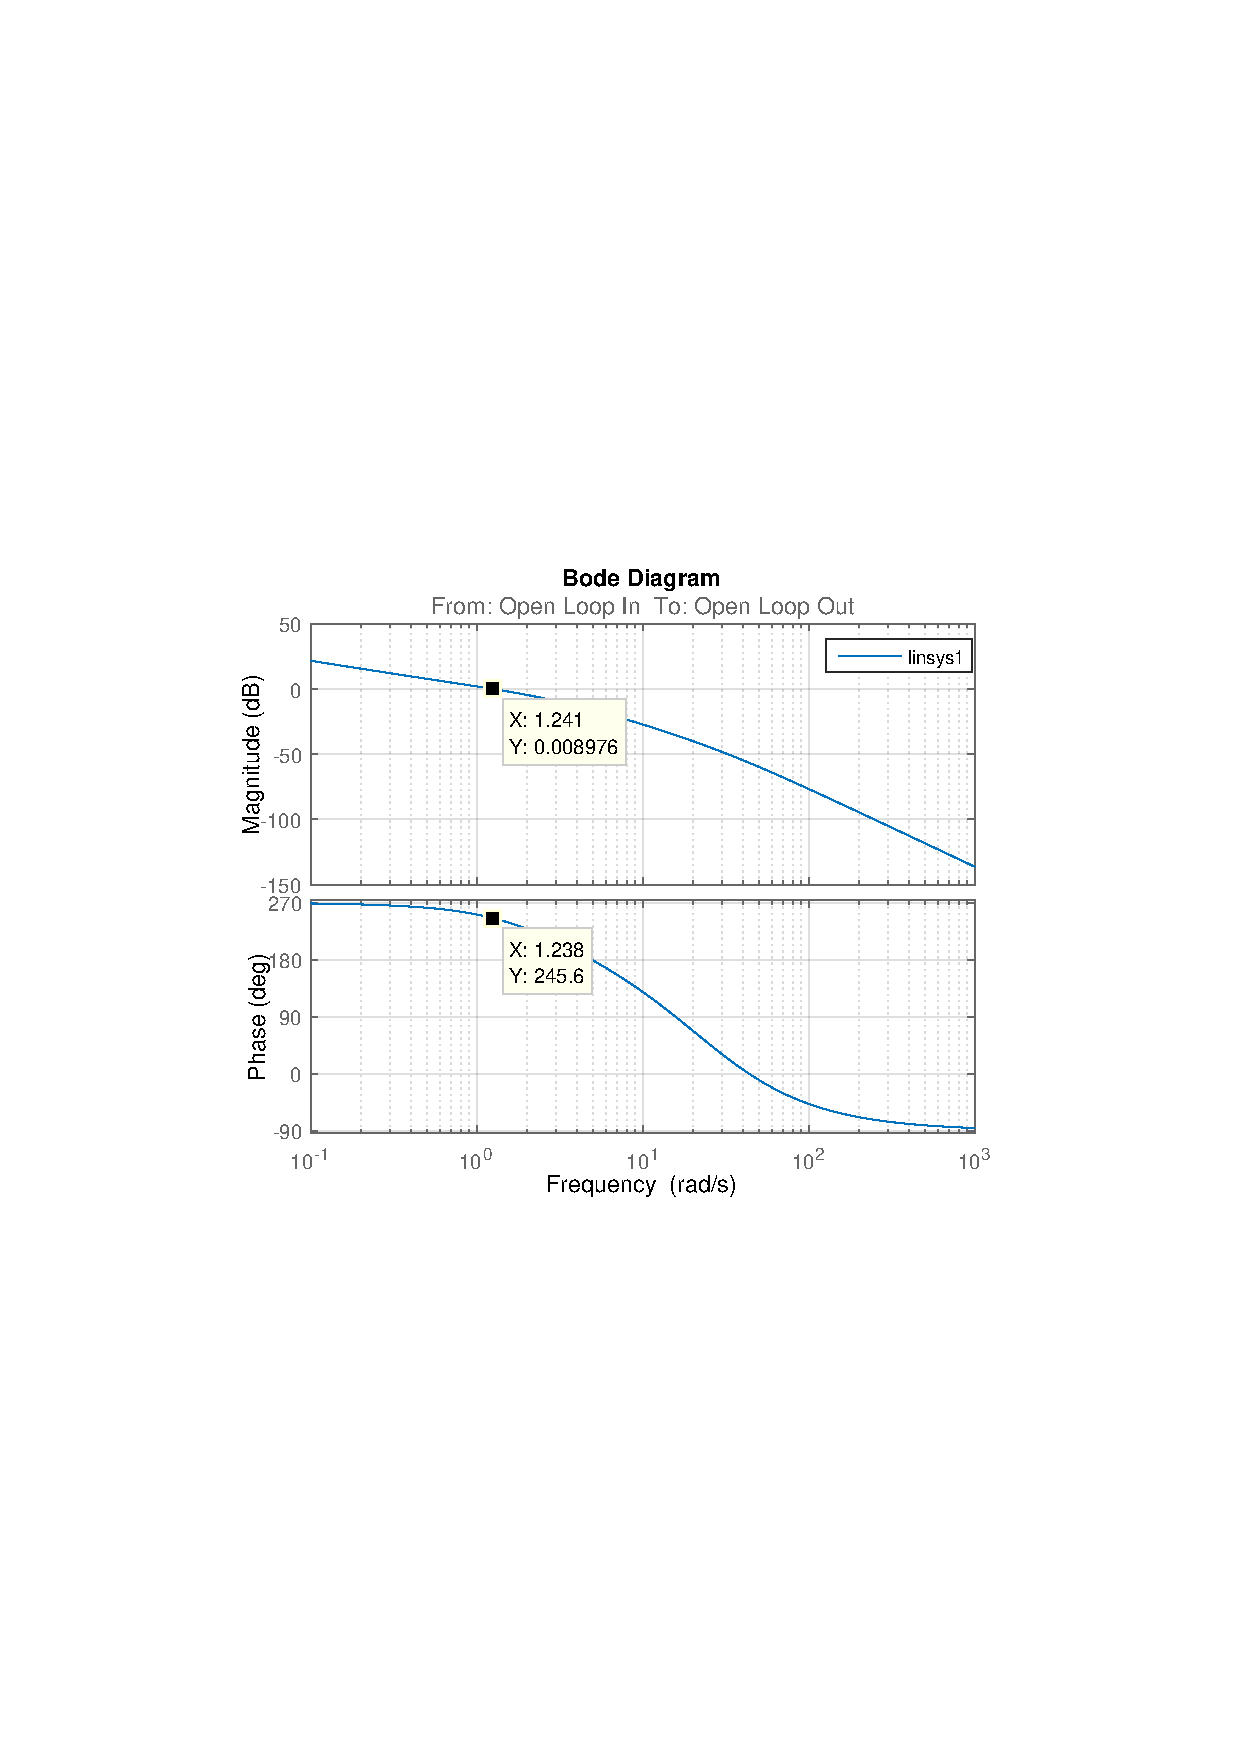
\includegraphics[width=1.4\textwidth]{figures/distanceBode2.pdf}
  }
  \caption{A plot illustrating a simulated step-response of the approximated velocity model (the blue line) and a measured step-response of the vehicle (the red line).}
  \label{SimulationSteeringB2}
\end{figure}
\begin{figure}[H]
  \centering
 	%Trim margins @:   left        bottom       right       top
 	\adjustbox{ trim = {.15\width} {.30\height} {.15\width} {.30\height}, clip }
  {
    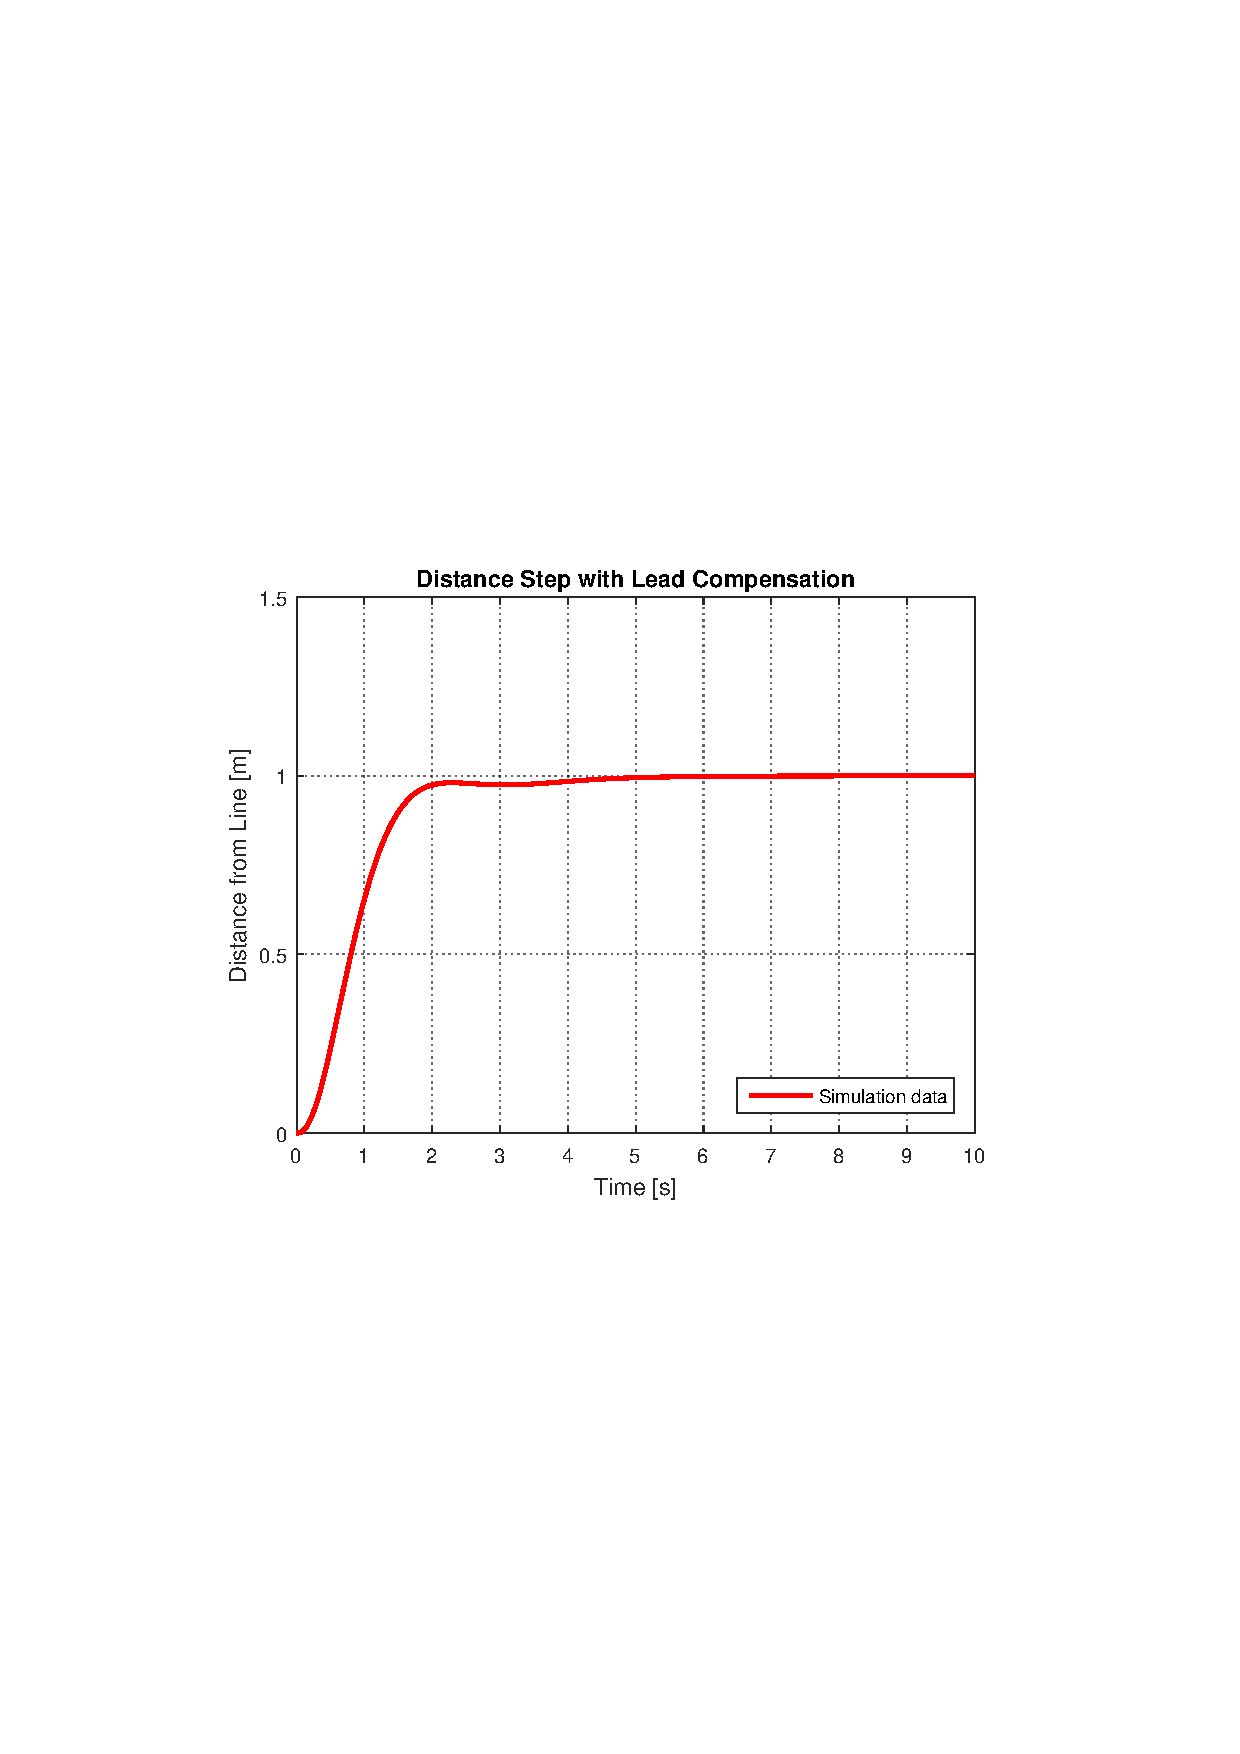
\includegraphics[width=1.4\textwidth]{figures/distanceStep3.pdf}
  }
  \caption{A plot illustrating a simulated step-response of the approximated velocity model (the blue line) and a measured step-response of the vehicle (the red line).}
  \label{SimulationSteeringP3}
\end{figure}